% 第1章第3节：平衡、周期与稳定性（平衡点与周期轨道；线性稳定与局部线性化；Lyapunov函数与吸引区域）。

\section{平衡、周期与稳定性}
\label{sec:dds-equilibria-stability}
\label{sec:dynamical-stability-sensitivity}

真实系统很少恰好从理想状态出发：初值有测量误差，运行中也会受到扰动。所以除了“轨迹去往哪里”，更要紧的是“出发点稍有偏差时，轨迹还去不去那里”。本节先找出不随时间改变的状态和周而复始的状态，再把“偏差不放大”“偏差最终消失”“偏差按几何速率消失”写成三种稳定性，最后按系统的结构给出判据：线性系统看谱半径，非线性系统先在平衡点处线性化，线性化不能回答时再寻找每步下降的Lyapunov函数。

\subsection{平衡点与周期轨道}
\label{sec:dds-equilibria-periodic}

\paragraph{平衡点}
温度模型在$x_*=2$处停住，是因为把$2$代入更新规则仍得到$2$。一般地，自治系统$x_{n+1}=F(x_n)$中满足
\begin{equation}
  F(x_*)=x_*
  \label{eq:dds-fixed-point}
\end{equation}
的状态称为\term{平衡点}（equilibrium point），也就是映射$F$的\term{不动点}（fixed point）。从平衡点出发的轨道永远停在那里。恒定输入的系统先把输入代入$F$，再按式~\eqref{eq:dds-fixed-point}求解，例如式~\eqref{eq:dds-forced-equilibrium}。

求平衡点是代数问题。Logistic映射~\eqref{eq:dds-logistic}的方程$x=rx(1-x)$化为$x\bigl(rx-(r-1)\bigr)=0$，解为$x=0$和$x_r=1-1/r$；后者在$r\geq1$时才落在$[0,1]$中。但求出平衡点只说明“停在那里就不会动”，没有说明附近的轨道会不会靠过来。$F(x)=2x$以$0$为平衡点，任何非零初值却都以倍增的速度离开它。平衡点的存在与它的稳定性必须分开讨论。

\paragraph{周期点与最小周期}
轨道还可能不停下来，而是周而复始。若$F^p(x)=x$（$p\geq1$），称$x$为周期$p$的点；使之成立的最小正整数$p$称为$x$的最小周期。此时轨道$x,F(x),\ldots,F^{p-1}(x)$两两不同，并按这个顺序循环，这$p$个点组成一条\term{周期轨道}（periodic orbit）。平衡点就是最小周期为$1$的点。

“最小”二字需要单独检查，因为平衡点满足$F^p(x_*)=x_*$对一切$p$成立。以Logistic映射的周期二为例，$F_r^2(x)=x$是关于$x$的四次方程，它的根包含两个平衡点$0$和$x_r$。把这两个因子除去，剩下二次方程
\[
  r^2x^2-r(r+1)x+(r+1)=0,\qquad
  x_\pm=\frac{(r+1)\pm\sqrt{(r+1)(r-3)}}{2r}.
\]
它在$r>3$时有两个不同的实根，且两根都不是平衡点，于是$\{x_-,x_+\}$是一条最小周期为二的轨道；$r=3$时两根重合为$x_r=2/3$，不再给出新的周期轨道。取$r=3.2$，算得$x_-\approx0.5130$、$x_+\approx0.7995$，代入可验证$F_{3.2}(x_-)=x_+$、$F_{3.2}(x_+)=x_-$。图~\ref{fig:dds-period-two-graph}把$F$与$F^2$画在一起：$F^2$与对角线有四个交点，其中两个是$F$的平衡点，另外两个就是周期二的点。

\begin{figure}[htbp]
  \centering
  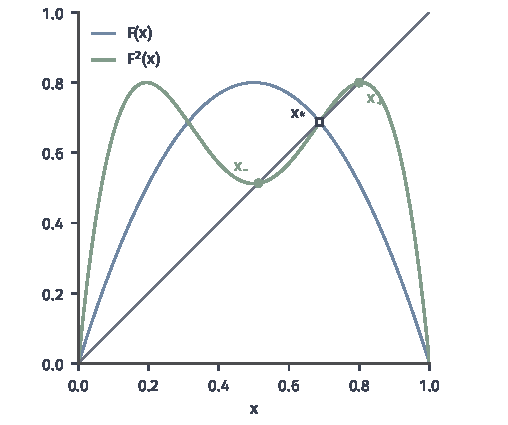
\includegraphics[width=80mm]{figures/03-optimization-evolution-and-signals/02-processes-and-trajectory-evolution/matplotlib/dds-period-two-graph/figure.pdf}
  \caption{$r=3.2$时Logistic映射$F$（蓝）与两步映射$F^2$（绿）。$F^2$与对角线的交点是$F^2$的不动点：$0$与$x_*=0.6875$同时也是$F$的不动点（方块标出$x_*$），$x_-\approx0.513$与$x_+\approx0.799$则组成最小周期为二的轨道。在$x_*$处$F^2$的斜率大于$1$，在$x_\pm$处斜率的绝对值小于$1$。}
  \label{fig:dds-period-two-graph}
\end{figure}

\paragraph{蛛网图：在函数图像上读轨道}
一维映射的轨道可以直接画在$F$的图像上，不必列出数表。在同一坐标系中画$y=F(x)$和对角线$y=x$。从$(x_0,x_0)$出发，竖直走到图像上的$(x_0,F(x_0))=(x_0,x_1)$，再水平走到对角线上的$(x_1,x_1)$，然后重复。竖直一步是“计算下一个值”，水平一步是“把输出当作新的输入”。这样画出的折线称为蛛网图。平衡点正是图像与对角线的交点。

图~\ref{fig:dds-cobweb}用蛛网图比较三种长期行为。(a)中$r=2.8$，折线绕着交点$x_r\approx0.643$一圈圈收紧，轨道收敛到平衡点；之所以是绕圈而不是单侧靠近，是因为该处图像的斜率$F'(x_r)=2-r=-0.8$为负，每一步都跳到平衡点的另一侧。(b)中$r=3.2$，折线不再收向交点，而是收向一个正方形，即周期二轨道$\{x_-,x_+\}$。(c)中$F(x)=x^2$在$x_*=1$处斜率为$2$，从$1.05$出发的轨道远离而去，从$0.95$出发的轨道离开$1$后滑向另一个平衡点$0$。

\begin{figure*}[htbp]
  \centering
  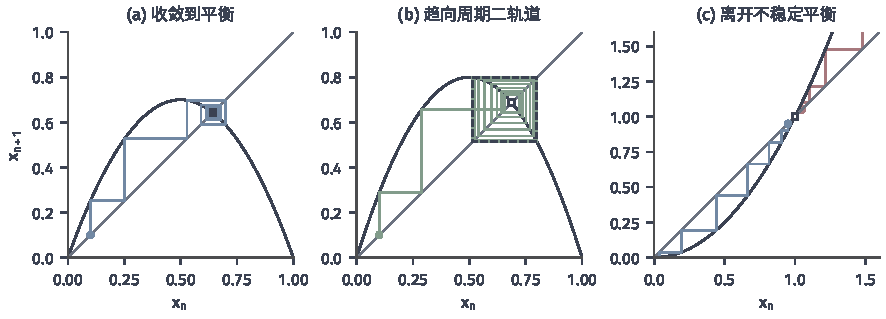
\includegraphics[width=150mm]{figures/03-optimization-evolution-and-signals/02-processes-and-trajectory-evolution/matplotlib/dds-cobweb/figure.pdf}
  \caption{三种长期行为的蛛网图。黑色曲线为$y=F(x)$，灰线为对角线，圆点为初值。(a)Logistic映射$r=2.8$、$x_0=0.1$，轨道绕平衡点$x_r=1-1/r$收紧。(b)$r=3.2$、$x_0=0.1$，轨道趋向虚线方框所示的周期二轨道，空心方块是已经失稳的平衡点$0.6875$。(c)$F(x)=x^2$，空心方块为$x_*=1$；红色从$1.05$出发并无界增长，蓝色从$0.95$出发并趋于$0$。}
  \label{fig:dds-cobweb}
\end{figure*}

\paragraph{周期轨道化为$p$步映射的不动点}
周期轨道的稳定性不需要新的理论。周期$p$的点是$G=F^p$的不动点，所以“附近的轨道是否回到这条周期轨道”可以转化为“$G$的这个不动点是否稳定”，下一小节的判据对$G$照样适用。对可微的一维映射，由链式法则，
\begin{equation}
  (F^p)'(x_0)=F'(x_{p-1})\,F'(x_{p-2})\cdots F'(x_0),
  \label{eq:dds-period-multiplier}
\end{equation}
右边是沿整条周期轨道的导数之积，与从哪一点开始无关。所以同一条周期轨道上的各点要么一起稳定，要么一起不稳定。这个乘积称为周期轨道的乘子，图~\ref{fig:dds-period-two-graph}中$F^2$在$x_\pm$处的斜率就是它。

\subsection{线性稳定与局部线性化}
\label{sec:dds-linear-stability}

\paragraph{三种稳定性}
设$X\subseteq\mathbb R^d$，$F:X\to X$连续，$\bm x_*$是平衡点，$\lVert\cdot\rVert$是$\mathbb R^d$上的一个范数。“偏差不放大”和“偏差最终消失”是两个不同的要求：前者限制整个未来的最大偏差，后者只管最终去向。再加上速度要求，就得到下面三种性质。

\begin{definition}[平衡点的稳定性]
\label{def:dds-stability}
\begin{enumerate}
  \item 若对每个$\varepsilon>0$存在$\delta>0$，使$\lVert\bm x_0-\bm x_*\rVert<\delta$蕴含$\lVert\bm x_n-\bm x_*\rVert<\varepsilon$对全部$n\geq0$成立，称$\bm x_*$在Lyapunov意义下\term{稳定}（stable）。
  \item 若$\bm x_*$稳定，且存在$r>0$，使$\lVert\bm x_0-\bm x_*\rVert<r$蕴含$\bm x_n\to\bm x_*$，称$\bm x_*$\term{渐近稳定}（asymptotically stable）。后一条件单独称为局部吸引。
  \item 若存在$r>0$、$C\geq1$与$0\leq q<1$，使$\lVert\bm x_0-\bm x_*\rVert<r$蕴含
  \[
    \lVert\bm x_n-\bm x_*\rVert\leq C\,q^n\,\lVert\bm x_0-\bm x_*\rVert,\qquad n\geq0,
  \]
  称$\bm x_*$\term{指数稳定}（exponentially stable）。
\end{enumerate}
若吸引条件或指数估计对全部$\bm x_0\in X$成立，相应地称为全局渐近稳定或全局指数稳定。
\end{definition}

量词的位置决定了各项的含义。稳定性是对每个容许偏差$\varepsilon$找初值半径$\delta$，要求整个未来都在$\varepsilon$之内，而不只是最终回来；吸引只要求最终趋于$\bm x_*$，途中可以走得很远；指数稳定要求常数$C,q$对邻域内全部初值统一。有限维空间上范数彼此等价，所以三种性质与所选范数无关，换范数只改变$\delta$和$C$。展示一条收敛的轨迹不能代替这些对整个邻域的陈述。

三个标量例子说明这些性质确实不同，原点都是平衡点。$x_{n+1}=x_n$：每个初值保持不动，原点稳定但不吸引。$x_{n+1}=x_n-x_n^3$：当$0<|x_0|\leq1$时$|x_{n+1}|=|x_n|(1-x_n^2)<|x_n|$，轨道单调地趋于$0$，原点渐近稳定；但衰减很慢，$x_0=0.5$时$x_{100}\approx0.069$、$x_{1000}\approx0.022$，大致与$1/\sqrt{2n}$相符，相邻两步之比$1-x_n^2\to1$，不存在统一的几何速率，所以不是指数稳定。$x_{n+1}=0.5x_n$：$|x_n|=0.5^n|x_0|$，全局指数稳定。

\paragraph{线性定常系统的谱判据}
对线性系统$\bm x_{n+1}=\bm A\bm x_n$，原点总是平衡点，轨道$\bm A^n\bm x_0$又有第~\ref{sec:dds-constant-coefficient}小节的显式描述，所以三种稳定性都能化成矩阵幂的条件。线性还带来一个简化：缩放初值等于缩放整条轨道，局部性质与全局性质没有区别。

\begin{theorem}[离散线性定常系统的稳定性判据]
\label{thm:dynamical-discrete-spectral-stability}
\label{thm:dds-spectral-stability}
设$\bm A\in\mathbb R^{d\times d}$，考察$\bm x_{n+1}=\bm A\bm x_n$的平衡点$\bm 0$。
\begin{enumerate}
  \item $\bm 0$稳定，当且仅当$\sup_{n\geq0}\lVert\bm A^n\rVert<\infty$。
  \item $\bm 0$渐近稳定，当且仅当$\rho(\bm A)<1$。此时$\bm 0$全局指数稳定：对任意$q\in(\rho(\bm A),1)$，存在$C\geq1$，使$\lVert\bm A^n\bm x_0\rVert\leq Cq^n\lVert\bm x_0\rVert$对全部$\bm x_0$与$n\geq0$成立。
\end{enumerate}
\end{theorem}

\begin{proof}
(1) 若$M=\sup_n\lVert\bm A^n\rVert<\infty$，对给定$\varepsilon$取$\delta=\varepsilon/M$，则$\lVert\bm x_0\rVert<\delta$时$\lVert\bm A^n\bm x_0\rVert\leq M\lVert\bm x_0\rVert<\varepsilon$。反之，若$\bm 0$稳定，取$\varepsilon=1$得到相应的$\delta$。对任意单位向量$\bm v$，$\lVert(\delta/2)\bm v\rVert<\delta$，所以$\lVert\bm A^n(\delta/2)\bm v\rVert<1$，即$\lVert\bm A^n\bm v\rVert<2/\delta$。对全部单位向量取上确界，得$\lVert\bm A^n\rVert\leq2/\delta$对全部$n$成立。

(2) 设$\rho(\bm A)<1$，任取$q\in(\rho(\bm A),1)$，由估计~\eqref{eq:dds-geometric-bound}得$\lVert\bm A^n\rVert\leq Cq^n$。这同时给出全局指数稳定、全局吸引，以及(1)中的有界性，从而渐近稳定。反之，设$\bm 0$渐近稳定，相应的吸引半径为$r$。对任意$\bm x_0\neq\bm 0$，$\bm y_0=(r/2)\bm x_0/\lVert\bm x_0\rVert$落在吸引邻域内，所以$\bm A^n\bm y_0\to\bm 0$；由线性，$\bm A^n\bm x_0=(2\lVert\bm x_0\rVert/r)\bm A^n\bm y_0\to\bm 0$。取$\bm x_0$为各个标准基向量，得$\bm A^n$的每一列趋于零，即$\bm A^n\to\bm 0$，再由第~\ref{sec:dds-constant-coefficient}小节所引的判据得$\rho(\bm A)<1$。
\end{proof}

谱半径严格小于$1$的矩阵称为\term{Schur稳定}（Schur stable）矩阵。定理说明，对线性系统，渐近稳定、全局渐近稳定和指数稳定是同一件事；它们都由特征值是否全部严格落在单位圆内决定。

谱半径等于$1$是临界情形，结果取决于单位圆上特征值的结构，不能只看谱半径。旋转矩阵$\bm R(\varphi)$的特征值是$\mathrm e^{\pm\mathrm i\varphi}$，$\lVert\bm R(\varphi)^n\rVert_2=1$，原点稳定但不吸引；$\operatorname{diag}(1,-1)$也稳定，轨道在两点之间来回翻转。而第~\ref{sec:dds-constant-coefficient}小节的$\bm J=\bigl[\begin{smallmatrix}1&1\\0&1\end{smallmatrix}\bigr]$同样只有特征值$1$，$\bm J^n$的右上角却是$n$，由定理的(1)，原点不稳定。一般结论是：$\sup_n\lVert\bm A^n\rVert<\infty$当且仅当$\rho(\bm A)\leq1$，且每个模为$1$的特征值的几何重数等于代数重数，也就是它对应的Jordan块都是一阶的；这可由Jordan标准形逐块计算矩阵幂得到，本章只用上面的二维例子说明机制。

时变系统不能套用这个判据。第~\ref{sec:dds-time-varying}小节交替使用两个幂零矩阵的例子中，每一步的谱半径都是$0$，轨道却每步翻倍。

\paragraph{非线性映射的局部线性化}
非线性映射一般没有显式解，但在平衡点附近，可微映射与它的线性部分相差很小。设$F$在$\bm x_*$的邻域内可微，记\term{Jacobian矩阵}（Jacobian matrix）$\bm J=DF(\bm x_*)$，则
\[
  F(\bm x)-\bm x_*=\bm J(\bm x-\bm x_*)+\bm\rho(\bm x),\qquad
  \frac{\lVert\bm\rho(\bm x)\rVert}{\lVert\bm x-\bm x_*\rVert}\to0\quad(\bm x\to\bm x_*).
\]
偏差$\bm e_n=\bm x_n-\bm x_*$近似满足线性递推$\bm e_{n+1}\approx\bm J\bm e_n$。用$\bm J$判断平衡点的稳定性，就是\term{线性化}（linearization）。可微、Jacobian矩阵与余项的性质可参考\BookChapterRef{chap:multivariate-calculus}{卷一“多元函数微分”章}。下面的定理说明，只要$\bm J$的谱不落在单位圆上，线性化给出的结论就是对的。

\begin{theorem}[线性化判据]
\label{thm:dds-linearization}
设$U\subseteq\mathbb R^d$为开集，$F:U\to\mathbb R^d$在平衡点$\bm x_*\in U$处可微，$\bm J=DF(\bm x_*)$。
\begin{enumerate}
  \item 若$\rho(\bm J)<1$，则$\bm x_*$指数稳定。
  \item 若$\bm J$有模大于$1$的特征值，则$\bm x_*$不稳定。
\end{enumerate}
\end{theorem}

\begin{proof}
(1) 取$\rho(\bm J)<q_1<q<1$。由第~\ref{sec:dds-constant-coefficient}小节所引的范数构造，存在$\mathbb R^d$上的范数$\lVert\cdot\rVert_*$，使$\bm J$在其诱导矩阵范数下满足$\lVert\bm J\rVert_*\leq q_1$。由可微性，存在$r>0$，使$\lVert\bm x-\bm x_*\rVert_*<r$时$\bm x\in U$且$\lVert\bm\rho(\bm x)\rVert_*\leq(q-q_1)\lVert\bm x-\bm x_*\rVert_*$。于是在这个球内
\[
  \lVert F(\bm x)-\bm x_*\rVert_*\leq\lVert\bm J\rVert_*\lVert\bm x-\bm x_*\rVert_*+(q-q_1)\lVert\bm x-\bm x_*\rVert_*\leq q\,\lVert\bm x-\bm x_*\rVert_*.
\]
右边小于$r$，所以$F$把球映回自身；归纳得$\lVert\bm x_n-\bm x_*\rVert_*\leq q^n\lVert\bm x_0-\bm x_*\rVert_*$。由范数等价，存在$c_1,c_2>0$使$c_1\lVert\cdot\rVert\leq\lVert\cdot\rVert_*\leq c_2\lVert\cdot\rVert$，于是对$\lVert\bm x_0-\bm x_*\rVert<r/c_2$有$\lVert\bm x_n-\bm x_*\rVert\leq(c_2/c_1)q^n\lVert\bm x_0-\bm x_*\rVert$，这就是指数稳定。

(2) 不妨设$\bm x_*=\bm 0$。记$\mu_0=\min\{|\lambda|:|\lambda|>1\}$，取$\mu\in(1,\mu_0)$使$\bm J$没有模等于$\mu$的特征值。按特征值的模大于或小于$\mu$，$\mathbb R^d$分解为两个$\bm J$不变子空间的直和$E_u\oplus E_c$，$E_u\neq\{\bm 0\}$；这是线性代数中按特征值分组的不变子空间分解。记$\bm J_u,\bm J_c$为$\bm J$在两个子空间上的限制，则$\bm J_u$可逆，$\rho(\bm J_u^{-1})<1/\mu$，$\rho(\bm J_c)<\mu$。取$1<b<a$使$\rho(\bm J_c)<b<\mu<a$且$\rho(\bm J_u^{-1})<1/a$，再像(1)那样在两个子空间上分别取范数，使$\lVert\bm J_c\bm v\rVert\leq b\lVert\bm v\rVert$、$\lVert\bm J_u\bm w\rVert\geq a\lVert\bm w\rVert$。把$\bm x=\bm w+\bm v$（$\bm w\in E_u$，$\bm v\in E_c$）的范数定义为$\lVert\bm w\rVert+\lVert\bm v\rVert$，并考虑锥形区域$K=\{\lVert\bm v\rVert\leq\lVert\bm w\rVert\}$。

令$\gamma=(a-b)/4$，取$r>0$使$\lVert\bm x\rVert<r$时$\bm x\in U$且余项满足$\lVert\bm\rho(\bm x)\rVert\leq\gamma\lVert\bm x\rVert$；按所取范数的定义，余项在$E_u$、$E_c$上的两个分量的范数都不超过$\lVert\bm\rho(\bm x)\rVert$。对$\bm x\in K$且$\lVert\bm x\rVert<r$，有$\lVert\bm x\rVert\leq2\lVert\bm w\rVert$，于是$F(\bm x)$的两个分量满足
\[
  \lVert\bm w'\rVert\geq a\lVert\bm w\rVert-2\gamma\lVert\bm w\rVert,\qquad
  \lVert\bm v'\rVert\leq b\lVert\bm v\rVert+2\gamma\lVert\bm w\rVert\leq(b+2\gamma)\lVert\bm w\rVert .
\]
因为$a-2\gamma=b+2\gamma=(a+b)/2>1$，所以$F(\bm x)\in K$且$\lVert\bm w'\rVert\geq\kappa\lVert\bm w\rVert$，$\kappa=(a+b)/2>1$。于是从$K$中任意小的非零初值（例如$\bm x_0=\bm w_0\in E_u$）出发，只要轨道还在半径$r$的球内，$E_u$分量就每步至少乘以$\kappa$，因而有限步内必然离开这个球。取$\varepsilon=r$，不存在满足稳定性定义的$\delta$。
\end{proof}

定理把非线性问题的大部分情形交给了线性代数。下面把它用在贯穿本节的Logistic映射上。

\begin{example}[Logistic映射的平衡点与周期二轨道]
\label{ex:dds-logistic-linearization}
$F_r'(x)=r(1-2x)$，在平衡点$x_r=1-1/r$处$F_r'(x_r)=2-r$。所以$1<r<3$时$|2-r|<1$，$x_r$指数稳定；$r>3$时$F_r'(x_r)<-1$，$x_r$不稳定，这正是图~\ref{fig:dds-cobweb}(a)(b)之间发生的变化。对周期二轨道，把定理用于$F_r^2$，由式~\eqref{eq:dds-period-multiplier}与$x_++x_-=(r+1)/r$、$x_+x_-=(r+1)/r^2$，
\[
  (F_r^2)'(x_\pm)=r^2(1-2x_+)(1-2x_-)=r^2-2r(r+1)+4(r+1)=-r^2+2r+4 .
\]
$r=3.2$时乘子为$0.16$，周期二轨道稳定，与蛛网图一致。第~\ref{sec:dds-bifurcation}小节将跟踪这个乘子随$r$的变化。
\end{example}

谱落在单位圆上时，线性化无法下结论，必须看高阶项。$x_{n+1}=x_n-x_n^3$与$x_{n+1}=x_n+x_n^3$在原点的导数都是$1$；前者原点渐近稳定（前面已经算过），后者从任何$x_0>0$出发都单调增长并离开原点，原点不稳定。同样的线性部分，长期行为相反。

\paragraph{长期衰减与瞬态放大}
谱判据描述$n\to\infty$时的行为，对有限步内发生什么说得很少。考察
\[
  \bm A_K=\begin{bmatrix}0.5&K\\0&0.5\end{bmatrix},\qquad
  \bm A_K^n=\begin{bmatrix}0.5^n&2nK\,0.5^{n}\\0&0.5^n\end{bmatrix}.
\]
无论$K$多大，谱半径都是$0.5$，原点全局指数稳定。从$\bm x_0=(0,1)^{\top}$出发，$K=4$时第一步就到达$(4,0.5)^{\top}$，欧氏长度约$4.03$，第二步约$4.01$，第三步约$3.00$，直到第六步才回到初始长度$1$以下（图~\ref{fig:dds-transient-growth}）。放大不来自输入，也不来自数值误差，而来自第二个坐标通过$K$对第一个坐标的持续推动，即前面Jordan块中多项式因子$n$的作用。

\begin{figure}[htbp]
  \centering
  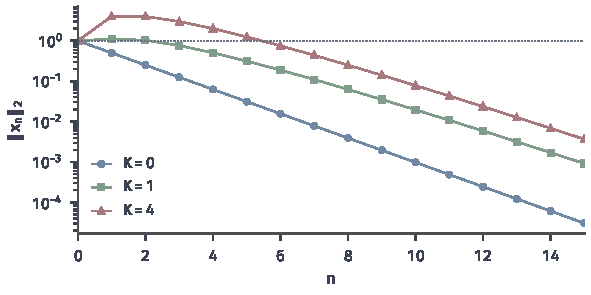
\includegraphics[width=100mm]{figures/03-optimization-evolution-and-signals/02-processes-and-trajectory-evolution/matplotlib/dds-transient-growth/figure.pdf}
  \caption{同一谱半径下的不同瞬态。对$\bm A_K=\bigl[\begin{smallmatrix}0.5&K\\0&0.5\end{smallmatrix}\bigr]$与$\bm x_0=(0,1)^{\top}$，画出$\lVert\bm A_K^n\bm x_0\rVert_2$，纵轴取对数，点线为初始长度$1$。三条曲线的谱半径都是$0.5$，长期斜率相同；$K=1$时第一步长度约$1.12$，$K=4$时前两步约$4.03$与$4.01$。}
  \label{fig:dds-transient-growth}
\end{figure}

$K\neq0$时$\bm A_K\bm A_K^{\top}\neq\bm A_K^{\top}\bm A_K$，矩阵不是\term{正规矩阵}（normal matrix）。正规矩阵可由正交矩阵对角化，满足$\lVert\bm A^n\rVert_2=\rho(\bm A)^n$，不会出现瞬态放大；非正规矩阵的特征方向不正交，甚至不够用，初值可能是几个很长、方向几乎相反的分量相消的结果，分量以不同速度衰减时相消被打破，长度便先增后减。工程上若中间状态不得越过某个边界，例如温度不得超过安全上限，仅凭谱半径小于$1$不能保证安全，还需要直接估计有限步的增益$\lVert\bm A^n\rVert$。

\subsection{Lyapunov函数与吸引区域}
\label{sec:dds-lyapunov}

\paragraph{换一把尺子：二次Lyapunov函数}
图~\ref{fig:dds-transient-growth}提出一个问题：既然欧氏长度不是每步下降，能不能换一种“长度”，使它沿每条轨道都严格下降？如果能，稳定性就可以一步一步地验证，而不必计算整个矩阵幂。对线性系统，自然的候选是二次型$V(\bm x)=\bm x^{\top}\bm P\bm x$，其中$\bm P\succ\bm0$对称正定，它的水平集是一族椭圆。沿$\bm x_{n+1}=\bm A\bm x_n$的一步变化为
\[
  V(\bm A\bm x)-V(\bm x)=\bm x^{\top}(\bm A^{\top}\bm P\bm A-\bm P)\bm x .
\]
要求它对每个非零$\bm x$为负，就是要求$\bm A^{\top}\bm P\bm A-\bm P$负定。

\begin{theorem}[离散Lyapunov方程]
\label{thm:dynamical-discrete-lyapunov-equation}
\label{thm:dds-discrete-lyapunov-equation}
设$\bm A\in\mathbb R^{d\times d}$。以下三条等价：
\begin{enumerate}
  \item $\rho(\bm A)<1$，即$\bm A$是Schur稳定矩阵；
  \item 对每个对称正定矩阵$\bm Q$，方程
  \begin{equation}
    \bm A^{\top}\bm P\bm A-\bm P=-\bm Q
    \label{eq:dds-discrete-lyapunov}
  \end{equation}
  在$\mathbb R^{d\times d}$中有唯一解$\bm P$，且$\bm P$对称正定；
  \item 存在对称正定矩阵$\bm P$与$\bm Q$满足方程~\eqref{eq:dds-discrete-lyapunov}。
\end{enumerate}
\end{theorem}

\begin{proof}
(1)$\Rightarrow$(2)：取$q\in(\rho(\bm A),1)$，由估计~\eqref{eq:dds-geometric-bound}，$\lVert(\bm A^{\top})^k\bm Q\bm A^k\rVert\leq\lVert\bm Q\rVert C^2q^{2k}$（矩阵范数取谱范数，$\lVert\bm A^{\top k}\rVert_2=\lVert\bm A^k\rVert_2$），所以级数
\[
  \bm P=\sum_{k=0}^{\infty}(\bm A^{\top})^k\bm Q\bm A^k
\]
绝对收敛。每一项对称，$\bm P$对称；首项$\bm Q$正定、其余各项半正定，故$\bm P\succeq\bm Q\succ\bm0$。代入验证：$\bm A^{\top}\bm P\bm A=\sum_{k\geq1}(\bm A^{\top})^k\bm Q\bm A^k=\bm P-\bm Q$。若$\bm P'$是另一个解（不必对称），差$\bm D=\bm P-\bm P'$满足$\bm D=\bm A^{\top}\bm D\bm A$，反复代入得$\bm D=(\bm A^{\top})^n\bm D\bm A^n\to\bm0$，故$\bm D=\bm0$。

(2)$\Rightarrow$(3)：取$\bm Q=\bm I$即可。

(3)$\Rightarrow$(1)：设$\lambda\in\mathbb C$是$\bm A$的特征值，$\bm v\in\mathbb C^d$为相应的非零特征向量，$\bm v^*$表示共轭转置。对方程~\eqref{eq:dds-discrete-lyapunov}左乘$\bm v^*$、右乘$\bm v$，由$\bm A\bm v=\lambda\bm v$得
\[
  (|\lambda|^2-1)\,\bm v^*\bm P\bm v=-\bm v^*\bm Q\bm v .
\]
实对称正定矩阵对非零复向量也给出正的二次型：写$\bm v=\bm a+\mathrm i\bm b$，则$\bm v^*\bm P\bm v=\bm a^{\top}\bm P\bm a+\bm b^{\top}\bm P\bm b>0$，对$\bm Q$同理。所以$|\lambda|^2-1<0$。这对每个特征值成立，故$\rho(\bm A)<1$。
\end{proof}

方程~\eqref{eq:dds-discrete-lyapunov}又称Stein方程，它是关于$\bm P$的线性方程组，规模较大时有利用Schur分解的专门解法，可参考\BookChapterRef{chap:linear-equations-and-optimization}{卷一“线性方程与矩阵方程”章}。小规模时可以手算，并且手算能看清每个未知数从哪个方程来。

\begin{example}[二阶Stein方程的手算]
\label{ex:dds-stein-by-hand}
取前面的$\bm A_1=\bigl[\begin{smallmatrix}0.5&1\\0&0.5\end{smallmatrix}\bigr]$、$\bm Q=\bm I$，设$\bm P=\bigl[\begin{smallmatrix}p&s\\s&t\end{smallmatrix}\bigr]$。方程逐元素给出
\[
  0.25p-p=-1,\qquad 0.5p+0.25s-s=0,\qquad p+s+0.25t-t=-1,
\]
依次解得$p=4/3$、$s=8/9$、$t=116/27\approx4.30$。$\bm P$的特征值约为$1.09$和$4.54$，确实正定。
\end{example}

这个$\bm P$给出了一把倾斜的尺子。图~\ref{fig:dds-lyapunov-ellipses}(a)画出$V$的若干水平椭圆和从$(0,1)^{\top}$出发的轨道：第一步到达$(1,0.5)^{\top}$，越出了单位圆，欧氏长度从$1$增至$1.118$；但它落在更内层的椭圆上，$V$从$4.30$降到$3.30$，恰好减少$\bm x_0^{\top}\bm Q\bm x_0=1$。(b)比较两种长度：$\sqrt V$每步下降，欧氏长度则先升后降。

\begin{figure}[htbp]
  \centering
  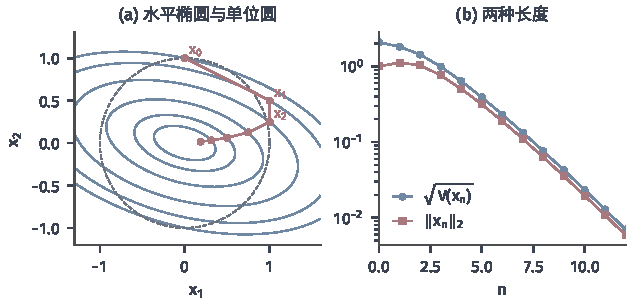
\includegraphics[width=107mm]{figures/03-optimization-evolution-and-signals/02-processes-and-trajectory-evolution/matplotlib/dds-lyapunov-ellipses/figure.pdf}
  \caption{二次Lyapunov函数作为倾斜的尺子。$\bm A=\bigl[\begin{smallmatrix}0.5&1\\0&0.5\end{smallmatrix}\bigr]$，$\bm P$由$\bm A^{\top}\bm P\bm A-\bm P=-\bm I$解出。(a)蓝色椭圆是轨道前六点所在的$V$水平集，虚线为单位圆，红点是从$\bm x_0=(0,1)^{\top}$出发的轨道：$\bm x_1$越出单位圆，却进入更内层的椭圆。(b)同一轨道的$\sqrt{V(\bm x_n)}$（蓝）与欧氏长度（红），纵轴取对数。}
  \label{fig:dds-lyapunov-ellipses}
\end{figure}

下降量还给出一个可验证的速度。记$p_+$、$p_-$为$\bm P$的最大、最小特征值，$q_-$为$\bm Q$的最小特征值。由$V(\bm x)\leq p_+\lVert\bm x\rVert_2^2$得$\bm x^{\top}\bm Q\bm x\geq q_-\lVert\bm x\rVert_2^2\geq(q_-/p_+)V(\bm x)$，所以
\[
  V(\bm x_{n+1})\leq\Bigl(1-\frac{q_-}{p_+}\Bigr)V(\bm x_n),\qquad
  \lVert\bm x_n\rVert_2\leq\sqrt{\frac{p_+}{p_-}}\Bigl(1-\frac{q_-}{p_+}\Bigr)^{n/2}\lVert\bm x_0\rVert_2 .
\]
例中$1-q_-/p_+\approx1-1/4.54\approx0.78$，图中$V$的第一步比值约为$0.77$，符合这一保证。因子$\sqrt{p_+/p_-}\approx2.04$正好容纳了欧氏长度的瞬态放大。这是Lyapunov函数给出的上界，不是最慢模态的精确衰减率：真实的长期速率由$\rho(\bm A)=0.5$决定，$V$的每步比值最终约为$0.25$。

\paragraph{Lyapunov函数的一般判据}
二次型只是一个特例。思想本身很朴素：找一个衡量“离平衡点多远”的非负量，证明它每走一步都不增加，最好是严格减少。梯度下降就是现成的例子。对可微目标$f$，若梯度满足$L$-Lipschitz条件，步长$0<\eta<2/L$时迭代$\bm x_{n+1}=\bm x_n-\eta\nabla f(\bm x_n)$满足
\[
  f(\bm x_{n+1})\leq f(\bm x_n)-\eta\Bigl(1-\frac{L\eta}{2}\Bigr)\lVert\nabla f(\bm x_n)\rVert_2^2 ,
\]
这一下降不等式见第~\ref{chap:opt-smooth}章。若$\bm x_*$是局部最小点，且附近没有别的驻点，那么$V=f-f(\bm x_*)$在$\bm x_*$附近正定，并且除$\bm x_*$外每步严格下降。目标函数本身就是迭代的Lyapunov函数。

设$\bm x_*$是连续映射$F$的平衡点，$G$是$\bm x_*$的一个邻域。连续函数$V:G\to[0,\infty)$若满足$V(\bm x_*)=0$且$V(\bm x)>0$对$\bm x\neq\bm x_*$成立，称为正定的。记一步增量
\[
  \Delta V(\bm x)=V(F(\bm x))-V(\bm x),
\]
它只在$F(\bm x)\in G$的点上有定义。

\begin{definition}[离散Lyapunov函数]
\label{def:dds-lyapunov-function}
若正定连续函数$V:G\to[0,\infty)$对一切满足$\bm x,F(\bm x)\in G$的$\bm x$有$\Delta V(\bm x)\leq0$，称$V$为$F$在$\bm x_*$处的\term{Lyapunov函数}（Lyapunov function）；若对这些$\bm x\neq\bm x_*$还有$\Delta V(\bm x)<0$，称为严格Lyapunov函数。
\end{definition}

$V$不必是能量或距离；它只需要在空间形状上把$\bm x_*$围起来（正定），并在动力学上不增（$\Delta V\leq0$）。正定性保证“$V$小”确实意味着“各个方向的偏差都小”，非增性保证轨道不能爬上更高的水平集。

\begin{theorem}[离散时间Lyapunov判据]
\label{thm:dds-lyapunov-criterion}
设$X\subseteq\mathbb R^d$，$F:X\to X$连续，$\bm x_*$为平衡点，$V$是$F$在$\bm x_*$的邻域$G$上的Lyapunov函数。
\begin{enumerate}
  \item $\bm x_*$稳定。
  \item 若$V$是严格Lyapunov函数，则$\bm x_*$渐近稳定。
  \item 若$G=X=\mathbb R^d$，$V$是严格Lyapunov函数，且$V(\bm x)\to\infty$当$\lVert\bm x\rVert\to\infty$，则$\bm x_*$全局渐近稳定。
\end{enumerate}
\end{theorem}

\begin{proof}
(1) 给定$\varepsilon>0$，不妨设闭球$\overline B_\varepsilon(\bm x_*)\subseteq G$。离散时间的轨道可能“跳过”球面，所以先用$F$的连续性控制一步的跨度：因$F(\bm x_*)=\bm x_*$，存在$\eta\in(0,\varepsilon]$，使$\lVert\bm x-\bm x_*\rVert<\eta$时$\lVert F(\bm x)-\bm x_*\rVert<\varepsilon$。紧环形$\{\eta\leq\lVert\bm x-\bm x_*\rVert\leq\varepsilon\}$上连续正函数$V$有正的最小值$m$。由$V$在$\bm x_*$连续，取$\delta\in(0,\eta)$使$\lVert\bm x-\bm x_*\rVert<\delta$时$V(\bm x)<m$。

设$\lVert\bm x_0-\bm x_*\rVert<\delta$。用归纳法证明$\lVert\bm x_n-\bm x_*\rVert<\eta$且$V(\bm x_n)<m$。$n=0$成立。若对$n$成立，则$\bm x_{n+1}=F(\bm x_n)$落在$B_\varepsilon(\bm x_*)\subseteq G$内，$\Delta V(\bm x_n)$有定义且不大于零，所以$V(\bm x_{n+1})\leq V(\bm x_n)<m$；而环形上$V\geq m$，所以$\bm x_{n+1}$不在环形中，只能满足$\lVert\bm x_{n+1}-\bm x_*\rVert<\eta$。于是整条轨道留在$B_\eta\subseteq B_\varepsilon$内。

(2) 按(1)对某个固定的$\varepsilon$取$\eta,\delta$，从$\lVert\bm x_0-\bm x_*\rVert<\delta$出发的轨道留在紧集$K_0=\overline B_\eta(\bm x_*)$中。$V(\bm x_n)$单调不增且非负，收敛到某个$c\geq0$。若$c>0$，轨道始终在紧集$K=\{\bm x\in K_0:V(\bm x)\geq c\}$中，$K$不含$\bm x_*$；连续函数$\Delta V$在$K$上处处为负，有最大值$-\gamma<0$，于是$V(\bm x_n)\leq V(\bm x_0)-n\gamma$，对大$n$为负，矛盾。所以$V(\bm x_n)\to0$。若$\bm x_n\not\to\bm x_*$，则有子列满足$\lVert\bm x_{n_k}-\bm x_*\rVert\geq\varepsilon'>0$，在紧集$K_0$中再取收敛子列，极限$\bm z\neq\bm x_*$满足$V(\bm z)=0$，与正定性矛盾。

(3) 径向无界性使每个子水平集$\{V\leq c\}$有界，又因$V$连续而是闭集，从而是紧集。从任意$\bm x_0$出发，$V(\bm x_n)\leq V(\bm x_0)$，轨道留在紧集$\{V\leq V(\bm x_0)\}$中，(2)中的论证逐字适用。
\end{proof}

线性化无法判断的临界例子，可以用这个判据处理。$x_{n+1}=x_n-x_n^3$取$V(x)=x^2$，
\[
  \Delta V(x)=(x-x^3)^2-x^2=x^4(x^2-2)<0,\qquad 0<|x|<\sqrt2 ,
\]
所以$V$是$(-\sqrt2,\sqrt2)$上的严格Lyapunov函数，原点渐近稳定。线性部分在这里只给出导数$1$，起作用的是三次项。

\paragraph{压缩映射：可计算的特例}
有一类映射，Lyapunov函数可以直接取为到不动点的距离。设$(X,d)$是完备度量空间，$F:X\to X$满足$d(F(x),F(y))\leq L\,d(x,y)$，$0\leq L<1$，称$F$为\term{压缩映射}（contraction mapping）。压缩映射定理断言：$F$有唯一不动点$x_*$，任意初值的轨道都收敛到它，并且
\begin{equation}
  d(x_n,x_*)\leq L^n d(x_0,x_*)\leq\frac{L^n}{1-L}\,d(x_0,x_1).
  \label{eq:dds-contraction-bound}
\end{equation}
用本节的语言，$V(x)=d(x,x_*)$每步至少乘以$L$，所以$x_*$全局指数稳定；第二个不等式只用已经算出的$x_0,x_1$，在不知道$x_*$时也能事先估计所需步数。定理的证明与误差估计可参考\BookChapterRef{chap:metric-spaces}{卷二“度量空间”章}。

定理的条件各有用处，缺一个就可能失效。下面先逐条核对一个满足全部条件的例子，再看缺少完备性时会发生什么。\begin{example}[余弦迭代]
\label{ex:dds-cosine-contraction}
取$X=[0,1]$：它是实数轴上的闭区间，因而完备；$\cos$把$[0,1]$映到$[\cos1,1]\subseteq[0,1]$，满足映回条件；由中值定理，$|\cos x-\cos y|\leq\sin1\cdot|x-y|$，$L=\sin1\approx0.841$。于是有唯一不动点$x_*\approx0.7391$。从$x_0=1$出发，先验估计~\eqref{eq:dds-contraction-bound}要求$n=20$时误差不超过约$0.092$，实际误差约为$10^{-4}$，估计偏保守但始终成立。
\end{example}

反过来，$F(x)=x/2$在$(0,1]$上是$L=1/2$的压缩映射且把$(0,1]$映回自身，轨道却趋向不在$(0,1]$中的$0$：$(0,1]$不完备，不动点不存在。

梯度下降在二次目标上恰好是压缩映射。$f(\bm x)=\frac12\bm x^{\top}\bm H\bm x$、$\bm H\succ\bm0$时，更新是$\bm x\mapsto(\bm I-\eta\bm H)\bm x$，而对称矩阵$\bm I-\eta\bm H$的谱范数为$\max_i|1-\eta\lambda_i(\bm H)|$，它在$0<\eta<2/\lambda_{\max}(\bm H)$时小于$1$。这一条件与线性谱判据给出的完全相同，因为对称矩阵的谱范数就等于谱半径，不存在瞬态放大。

\paragraph{子水平集与吸引区域}
定理~\ref{thm:dds-lyapunov-criterion}的(1)(2)只保证“足够近”的初值，没有说多近才算够近。Lyapunov函数还能回答这个问题：它的子水平集给出一块可以证明的吸引区域。

\begin{theorem}[子水平集估计吸引区域]
\label{thm:dds-sublevel-basin}
设$F:\mathbb R^d\to\mathbb R^d$连续，$\bm x_*$为平衡点，$V:\mathbb R^d\to[0,\infty)$连续且正定。若对某个$c>0$，子水平集$\Omega_c=\{\bm x:V(\bm x)\leq c\}$是紧集，并且$\Delta V(\bm x)<0$对一切$\bm x\in\Omega_c\setminus\{\bm x_*\}$成立，则$\Omega_c$正向不变，且从$\Omega_c$出发的每条轨道都收敛到$\bm x_*$。
\end{theorem}

\begin{proof}
若$\bm x\in\Omega_c$且$\bm x\neq\bm x_*$，则$V(F(\bm x))<V(\bm x)\leq c$；又$F(\bm x_*)=\bm x_*\in\Omega_c$。所以$F(\Omega_c)\subseteq\Omega_c$。从$\Omega_c$出发的轨道留在紧集$\Omega_c$中，定理~\ref{thm:dds-lyapunov-criterion}(2)证明中的论证（以$\Omega_c$代替$K_0$）给出$V(\bm x_n)\to0$与$\bm x_n\to\bm x_*$。
\end{proof}

这个定理的价值在于把“轨道会不会逃逸”的问题，变成“$\Delta V$在一个有界集合上是否为负”的检查，而后者不需要计算任何轨道。考察非线性映射
\[
  F(x_1,x_2)=(0.5x_1+x_2,\ 0.5x_2+x_1^2),
\]
它在原点的线性部分正是前面的$\bm A_1$，所以由定理~\ref{thm:dds-linearization}，原点指数稳定。沿用同一个$\bm P$，取$V(\bm x)=\bm x^{\top}\bm P\bm x$。原点附近二次项起主导作用，$\Delta V\approx-\lVert\bm x\rVert_2^2<0$；离原点较远时，非线性项$x_1^2$可能使$\Delta V\geq0$。在网格上数值寻找$\Delta V\geq0$的点上$V$的最小值，约为$c^*\approx0.173$。取稍小的$c=0.164$，椭圆$\Omega_c$内处处$\Delta V<0$，由定理，$\Omega_c$中每个初值的轨道都收敛到原点。

\begin{figure}[htbp]
  \centering
  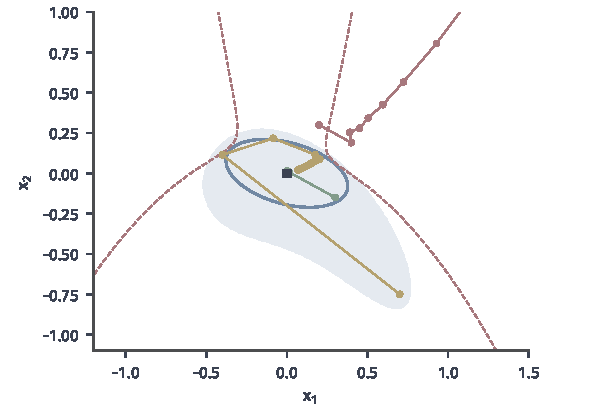
\includegraphics[width=100mm]{figures/03-optimization-evolution-and-signals/02-processes-and-trajectory-evolution/matplotlib/dds-basin-estimate/figure.pdf}
  \caption{子水平集给出的吸引区域。映射$F(x_1,x_2)=(0.5x_1+x_2,\,0.5x_2+x_1^2)$，$V=\bm x^{\top}\bm P\bm x$沿用图~\ref{fig:dds-lyapunov-ellipses}的$\bm P$。浅蓝区域是数值估计的吸引域（$700\times560$网格，迭代$200$步后距原点小于$10^{-6}$）；红色虚线是$\Delta V=0$的曲线；蓝色椭圆$\Omega_c$（$c=0.164$）完全落在$\Delta V<0$的一侧。绿色轨道从椭圆内出发；黄色轨道从椭圆外、吸引域内出发，也收敛；红色轨道从吸引域外出发并逃逸。}
  \label{fig:dds-basin-estimate}
\end{figure}

图~\ref{fig:dds-basin-estimate}把证明得到的椭圆和数值估计的真实吸引域画在一起。椭圆是一个保守的估计：吸引域在右下方伸得更远，黄色轨道从椭圆外出发同样收敛，只是这一点没有被这个$V$证明。估计的大小取决于$V$的选择，换一个$\bm Q$或者非二次的$V$可能证出更大的区域。$c^*$本身是网格上的数值估计；严格的证明需要在$\Omega_c$上对$\Delta V<0$给出解析或区间算术的验证，网格检查只是提示。

\paragraph{非严格下降}
若只知道$\Delta V\leq0$，定理只保证稳定，不保证收敛。旋转$\bm x_{n+1}=\bm R(\varphi)\bm x_n$取$V=\lVert\bm x\rVert_2^2$，$\Delta V\equiv0$，非零初值的轨道永远在圆周上转动。能量不增加，不等于能量会耗尽。但非严格下降仍然提供了信息：轨道最终只能停留在不再下降的地方。

\begin{theorem}[非严格下降时的极限点]
\label{thm:dds-lasalle}
设$\Omega\subseteq\mathbb R^d$紧且正向不变，$F$在$\Omega$上连续，$V:\Omega\to\mathbb R$连续，且$\Delta V(\bm x)\leq0$对一切$\bm x\in\Omega$成立。记$E=\{\bm x\in\Omega:\Delta V(\bm x)=0\}$。则对任意$\bm x_0\in\Omega$，轨道的每个极限点$\bm z$都满足：$F^k(\bm z)\in E$对全部$k\geq0$成立。特别地，若$E$中唯一一个整条正向轨道都留在$E$内的点是平衡点$\bm x_*$，则$\bm x_n\to\bm x_*$。
\end{theorem}

\begin{proof}
$V(\bm x_n)$单调不增，又因$V$在紧集上有下界而收敛到某个$c$。设子列$\bm x_{n_j}\to\bm z$。对固定的$k$，$F^k$连续，所以$\bm x_{n_j+k}=F^k(\bm x_{n_j})\to F^k(\bm z)$，从而$V(F^k(\bm z))=\lim_jV(\bm x_{n_j+k})=c$。这对每个$k$成立，于是$\Delta V(F^k(\bm z))=V(F^{k+1}(\bm z))-V(F^k(\bm z))=0$，即$F^k(\bm z)\in E$。最后一句：在所述条件下每个极限点都等于$\bm x_*$；若$\bm x_n\not\to\bm x_*$，在紧集$\Omega$中可以取出一个离$\bm x_*$至少$\varepsilon$的收敛子列，其极限是不等于$\bm x_*$的极限点，矛盾。
\end{proof}

这个结论是LaSalle不变性原理的离散形式，第~\ref{sec:dds-limit-sets}小节引入极限集合后还会用更紧凑的语言重述它。看一个例子：$F(\bm x)=\bm R(\varphi)\bm D\bm x$，$\bm D=\operatorname{diag}(1,1/2)$，即先把第二坐标减半、再旋转$\varphi$。取$V=\lVert\bm x\rVert_2^2$，旋转不改变长度，所以
\[
  \Delta V(\bm x)=\lVert\bm D\bm x\rVert_2^2-\lVert\bm x\rVert_2^2=-\tfrac34x_2^2\leq0 .
\]
$V$只在第二坐标上耗散，$E$是整条横轴$\{x_2=0\}$，比平衡点大得多。但横轴上的点$(z_1,0)$一步后到达$z_1(\cos\varphi,\sin\varphi)$，只要$\sin\varphi\neq0$且$z_1\neq0$，它就离开了横轴。所以整条轨道都留在$E$中的点只有原点，任何闭球都是紧的正向不变集，由定理全部轨道收敛到原点。旋转把横轴上的“能量”不断转到会耗散的方向，这正是非严格下降仍能导致收敛的机制。反之，$\varphi=0$时$F=\bm D$，横轴上每个点都是平衡点，轨道$\bm x_n=(x_{0,1},2^{-n}x_{0,2})$收敛到横轴上的某一点，而不是原点。
